\section{Giới thiệu đề tài}

\subsection{Bối cảnh thực tiễn}

Trong bối cảnh chăm sóc sức khỏe hiện đại, nhu cầu tiếp cận thông tin y tế đáng tin cậy và kịp thời đang gia tăng mạnh mẽ. Người dân thường gặp nhiều thách thức trong việc quản lý sức khỏe cá nhân, đặc biệt là khả năng nhận diện và đánh giá đúng các triệu chứng ban đầu, phân biệt các dấu hiệu cảnh báo cần can thiệp y tế khẩn cấp, và tìm kiếm nguồn thông tin y khoa chính thống giữa lượng lớn thông tin không được kiểm chứng trên internet.

Bên cạnh đó, việc theo dõi các chỉ số sức khỏe quan trọng như huyết áp, đường huyết, hoặc các triệu chứng của bệnh mãn tính đòi hỏi sự hiểu biết về xu hướng biến thiên và khả năng diễn giải kết quả một cách chính xác. Tại nhiều khu vực, khả năng tiếp cận bác sĩ chuyên khoa vẫn còn hạn chế, trong khi việc tự điều trị thiếu cơ sở khoa học có thể dẫn đến nguy cơ lạm dụng thuốc hoặc trì hoãn điều trị khi cần thiết.

Những thách thức này tạo ra nhu cầu cấp thiết về một hệ thống hỗ trợ y tế thông minh, có khả năng cung cấp thông tin chính xác, hướng dẫn sơ bộ về các vấn đề sức khỏe, và hỗ trợ theo dõi tình trạng sức khỏe một cách có hệ thống và khoa học.

\subsection{Bối cảnh công nghệ}

Sự phát triển vượt bậc của trí tuệ nhân tạo trong những năm gần đây, đặc biệt là công nghệ AI đa tác nhân (multi-agent) và AI đa phương thức (multimodal), đã mở ra những cơ hội mới trong lĩnh vực chăm sóc sức khỏe số. Các công nghệ này cho phép xây dựng các hệ thống có khả năng điều phối linh hoạt nhiều tác vụ y khoa phức tạp như hỏi đáp chuyên môn, truy xuất tri thức y khoa, phân tích hình ảnh y tế, và tìm kiếm thông tin thời gian thực trong một quy trình thống nhất và có tổ chức.

Đặc biệt, khả năng kết hợp tri thức có cấu trúc thông qua Knowledge Graph với các tài liệu y khoa không cấu trúc thông qua công nghệ RAG (Retrieval-Augmented Generation), cùng với tìm kiếm web có kiểm soát, đã tạo ra những giải pháp có độ tin cậy cao và khả năng cập nhật thông tin liên tục. Hơn nữa, khả năng xử lý dữ liệu đa phương thức (văn bản, hình ảnh, âm thanh) và duy trì ngữ cảnh trong các cuộc hội thoại dài cho phép tạo ra các chuỗi hỏi đáp đa bước (multi-hop QA) nhằm thu thập đầy đủ thông tin lâm sàng trước khi đưa ra khuyến nghị.

Các công nghệ AI hiện đại cũng hỗ trợ việc theo dõi các chỉ số sức khỏe một cách thông minh, có khả năng tổng hợp báo cáo tự động và cá nhân hóa ngưỡng cảnh báo dựa trên dữ liệu cá nhân của từng người dùng, từ đó nâng cao hiệu quả quản lý sức khỏe cá nhân.

\subsection{Mục tiêu}

Mục tiêu chính của đề tài là xây dựng một \textbf{Hệ thống Trợ lý Y tế Đa tác nhân và Đa phương thức} với các chức năng hỗ trợ toàn diện:

\textbf{Chẩn đoán gợi ý và tư vấn thông minh:} Hệ thống có khả năng phân tích triệu chứng dựa trên thông tin văn bản và hình ảnh, kết hợp với cơ chế hỏi đáp đa bước (multi-hop QA) để đảm bảo thu thập đầy đủ dữ liệu lâm sàng cần thiết trước khi đưa ra kết luận hoặc khuyến nghị. Quá trình này được thiết kế để mô phỏng cách tiếp cận có hệ thống của các chuyên gia y tế trong việc thu thập thông tin bệnh sử.

\textbf{Theo dõi và quản lý sức khỏe liên tục:} Hệ thống cung cấp khả năng theo dõi các chỉ số sức khỏe quan trọng như huyết áp, đường huyết, và các thông số sinh tồn khác. Nó có thể tổng hợp xu hướng biến thiên theo thời gian, sinh ra các báo cáo y khoa có cấu trúc chuyên nghiệp, và đưa ra các gợi ý cá nhân hóa về ngưỡng cảnh báo dựa trên đặc điểm riêng của từng người dùng.

\textbf{Đảm bảo an toàn và độ tin cậy:} Hệ thống được trang bị các cơ chế kiểm duyệt đầu ra (guardrails) để đảm bảo tính chính xác và an toàn của thông tin. Khi cần thiết, hệ thống yêu cầu xác nhận từ con người (human-in-the-loop) và luôn trích dẫn nguồn thông tin khi phù hợp để người dùng có thể kiểm chứng.

Quan trọng nhất, hệ thống được thiết kế với tuyên bố rõ ràng rằng nó mang tính chất hỗ trợ thông tin và \textit{không thay thế} vai trò tư vấn, chẩn đoán, và điều trị chuyên môn của các bác sĩ và nhân viên y tế được đào tạo bài bản.

\vspace{0.5cm}
\section{Giải pháp đề xuất và Kiến trúc hệ thống}

\subsection{Multi-Agent Medical Assistant}

Giải pháp được đề xuất là một \textbf{kiến trúc đa tác nhân tiên tiến} sử dụng phương pháp điều phối bằng đồ thị (graph-based orchestration) để xử lý thông tin đa phương thức một cách hiệu quả và chính xác. Kiến trúc này được thiết kế để tối ưu hóa việc phân chia công việc giữa các tác nhân chuyên biệt, đảm bảo mỗi loại yêu cầu được xử lý bởi thành phần có năng lực phù hợp nhất.

\textbf{Decision Agent (Tác nhân Điều phối Trung tâm):} Đây là bộ não của hệ thống, có nhiệm vụ phân tích yêu cầu người dùng và ngữ cảnh cuộc hội thoại để định tuyến đến tác nhân chuyên biệt phù hợp. Nó hỗ trợ kiểm soát luồng xử lý, ghi nhớ lịch sử hội thoại và duy trì trạng thái của toàn bộ hệ thống, đảm bảo tính nhất quán và liên tục trong quá trình tương tác.

\textbf{Text Module với Khả năng Hỏi đáp Đa bước:} Module này được trang bị cơ chế Multi-hop QA tiên tiến, cho phép hệ thống chủ động đặt các câu hỏi bổ sung một cách có hệ thống để thu thập thông tin chi tiết về thời gian xuất hiện triệu chứng, mức độ nghiêm trọng, vị trí cụ thể, các triệu chứng kèm theo, tiền sử bệnh lý, và thuốc đang sử dụng. Quá trình này tiếp tục cho đến khi có đủ thông tin cốt lõi để đưa ra suy luận chẩn đoán gợi ý có độ tin cậy cao.

Module cũng tích hợp khả năng truy xuất song song từ cả RAG (tài liệu y khoa trong vector database) và Knowledge Graph (tri thức cấu trúc thông qua Cypher/Neo4j) để tăng cường độ bao phủ thông tin. Khi ngữ cảnh nội bộ chưa đủ tin cậy hoặc cần cập nhật, hệ thống tự động chuyển sang Web Search có kiểm soát để tìm kiếm thông tin mới nhất từ các nguồn uy tín.

\textbf{Vision Module với Khả năng Phân tích Hình ảnh Chuyên sâu:} Module này có khả năng nhận diện loại ảnh y tế và thực hiện chẩn đoán tổng quát bằng các mô hình ngôn ngữ đa phương thức lớn (MLLM). Đặc biệt, nó được trang bị các công cụ phân vùng chuyên biệt cho tổn thương da (sử dụng kiến trúc U-Net) và polyp nội soi (sử dụng DeepLabV3+), có khả năng sinh ra các ảnh overlay trực quan dễ diễn giải và tóm tắt kết quả kèm theo các khuyến nghị theo dõi cụ thể.

\textbf{Patient Database Agent (Tác nhân Quản lý Dữ liệu Bệnh nhân):} Đây là thành phần chuyên biệt cho việc theo dõi và tổng hợp thông tin sức khỏe dài hạn. Nó có khả năng ghi nhận các biểu mẫu patient intake có cấu trúc, lưu trữ và quản lý hồ sơ bệnh nhân, và truy xuất thông tin theo từng cá nhân cụ thể.

Đặc biệt quan trọng là khả năng theo dõi các chỉ số sức khỏe như huyết áp, tổng hợp xu hướng biến thiên theo ngày, phân tích độ biến thiên (variability), đánh giá đáp ứng điều trị (treatment response), và tự động sinh ra các báo cáo y khoa chuyên nghiệp định dạng Markdown. Hệ thống cũng có khả năng đưa ra các ngưỡng cảnh báo được cá nhân hóa dựa trên đặc điểm riêng của từng bệnh nhân.

\textbf{Guardrails và Human Validation:} Hệ thống được trang bị các cơ chế kiểm soát chất lượng đầu ra nghiêm ngặt, bao gồm việc thêm các tuyên bố an toàn và yêu cầu xác nhận từ người dùng hoặc nhân viên y tế khi nội dung có yếu tố rủi ro cao. Cách tiếp cận này đảm bảo có đủ dữ liệu trước khi đưa ra chẩn đoán gợi ý, ưu tiên tính an toàn và độ tin cậy, đồng thời hỗ trợ theo dõi sức khỏe liên tục và báo cáo tổng hợp chuyên nghiệp.

\subsection{Chức năng cơ bản}

Hệ thống Multi-Agent Medical Assistant cung cấp một bộ chức năng toàn diện được thiết kế để đáp ứng đa dạng nhu cầu chăm sóc sức khỏe của người dùng:

\textbf{Hỏi đáp Y tế Chuyên nghiệp:} Hệ thống có khả năng trả lời các câu hỏi y khoa phổ biến dựa trên cơ sở tri thức nội bộ phong phú và các tài liệu chuyên ngành được kiểm chứng. Mọi thông tin đều được trích dẫn nguồn rõ ràng khi phù hợp, đảm bảo tính minh bạch và khả năng kiểm chứng.

\textbf{Tư vấn Theo Triệu chứng với Multi-hop QA:} Đây là một trong những tính năng tiên tiến nhất của hệ thống. Thay vì chỉ phản hồi dựa trên thông tin ban đầu, hệ thống chủ động thu thập có hệ thống các trường thông tin cốt lõi bao gồm thời gian xuất hiện, mức độ nghiêm trọng, vị trí cụ thể, các triệu chứng kèm theo, tiền sử bệnh lý, và thuốc đang sử dụng. Khi thông tin đã đầy đủ, hệ thống sử dụng RAG và Knowledge Graph để suy luận chẩn đoán gợi ý và đưa ra khuyến nghị theo dõi. Trong trường hợp thông tin chưa đủ, hệ thống tiếp tục đặt câu hỏi bổ sung hoặc chuyển sang Web Search có kiểm soát.

\textbf{Phân tích Hình ảnh Y tế Chuyên sâu:} Vision Module có khả năng phân loại ảnh y tế và thực hiện chẩn đoán tổng quát bằng các mô hình AI tiên tiến. Đặc biệt, hệ thống có thể thực hiện phân vùng tổn thương da và polyp nội soi một cách chính xác, sinh ra các ảnh overlay trực quan và tóm tắt kết quả dễ hiểu cho người dùng không chuyên.

\textbf{Tra cứu Thông tin Y khoa Toàn diện:} Hệ thống cung cấp khả năng tra cứu thông tin về bệnh tật, thuốc men, và triệu chứng thông qua cả Knowledge Graph và tài liệu RAG. Nó ưu tiên nội dung tiếng Việt và bối cảnh lâm sàng phù hợp với điều kiện y tế tại Việt Nam.

\textbf{Theo dõi Chỉ số và Báo cáo Chuyên nghiệp:} Một trong những tính năng nổi bật là khả năng tạo báo cáo xu hướng và ngưỡng cảnh báo được cá nhân hóa cho các chỉ số như huyết áp. Hệ thống có thể phân tích circadian pattern (nhịp sinh học), độ biến thiên (variability), và đáp ứng điều trị (treatment response). Các giao diện và endpoint chuyên biệt như \texttt{/api/blood-pressure-report} và \texttt{/api/generate-bp-medical-report} được thiết kế để phục vụ việc tổng hợp dữ liệu và xuất báo cáo chuyên nghiệp.

\textbf{Quản lý Hồ sơ Bệnh nhân:} Hệ thống có khả năng ghi nhận các biểu mẫu theo dõi bệnh (patient intake) có cấu trúc, cập nhật hồ sơ bệnh nhân theo thời gian, và truy xuất thông tin về các bệnh đang hoạt động theo từng bệnh nhân cụ thể.

\textbf{Đảm bảo An toàn và Tuân thủ:} Mọi đầu ra của hệ thống đều được kiểm duyệt nghiêm ngặt, có cảnh báo khi phát hiện dấu hiệu nguy hiểm, và luôn nhấn mạnh vai trò tham khảo của AI cũng như khuyến nghị khám bác sĩ khi cần thiết. Điều này đảm bảo hệ thống hoạt động một cách có trách nhiệm và an toàn.

\section{Kiến trúc hệ thống}

\subsection{Kiến trúc tổng quan}

\begin{figure}[H]
    \centering
    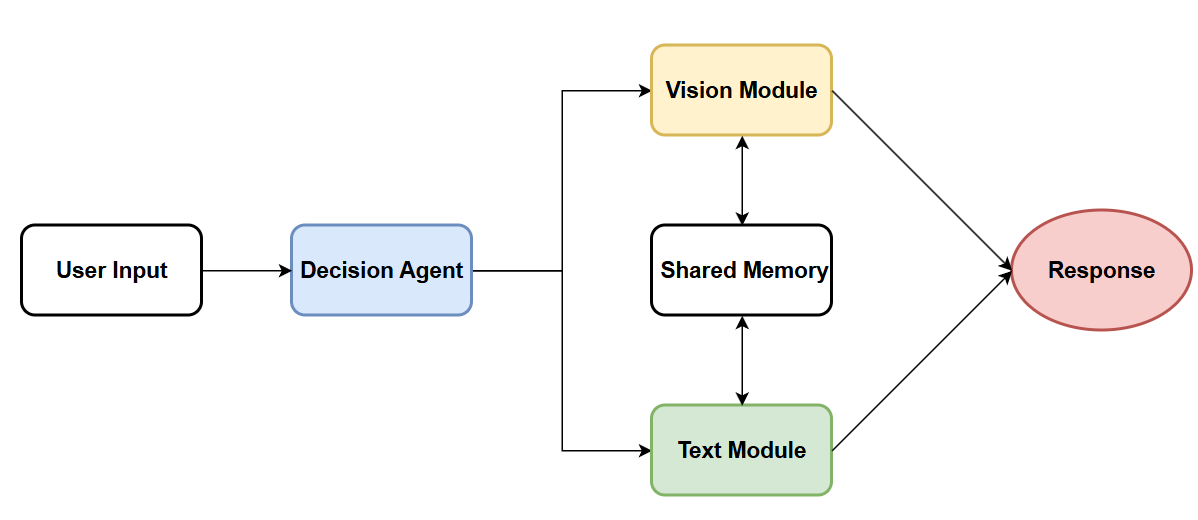
\includegraphics[width=0.8\textwidth]{images/tong_quan.png}
    \caption{Kiến trúc tổng quan hệ thống Multi-Agent Medical Assistant}
    \label{fig:system-overview}
\end{figure}

Hệ thống gồm 2 Module chính:

\textbf{Vision Module:} Thành phần này chịu trách nhiệm xử lý và kết hợp các dạng thông tin hình ảnh. Nó có khả năng nhận diện loại ảnh, áp dụng các mô hình phù hợp để phân tích, và đưa ra kết quả phân tích. Thông tin phân tích từ Vision Agent cũng được lưu trữ trong bộ nhớ chia sẻ (shared memory) để phục vụ cho các lần hỏi sau, giúp hệ thống có thể duy trì ngữ cảnh và cải thiện độ chính xác của các phản hồi.

\textbf{Text Module:} Thành phần này tập trung vào việc trích xuất các thông tin cần thiết từ các nguồn văn bản, tổng hợp và đưa ra kết quả. Text Agent đóng vai trò quan trọng trong việc xử lý các truy vấn dựa trên văn bản và cung cấp thông tin y khoa từ các nguồn đáng tin cậy.


\subsection{Kiến trúc chi tiết}

\begin{figure}[H]
    \centering
    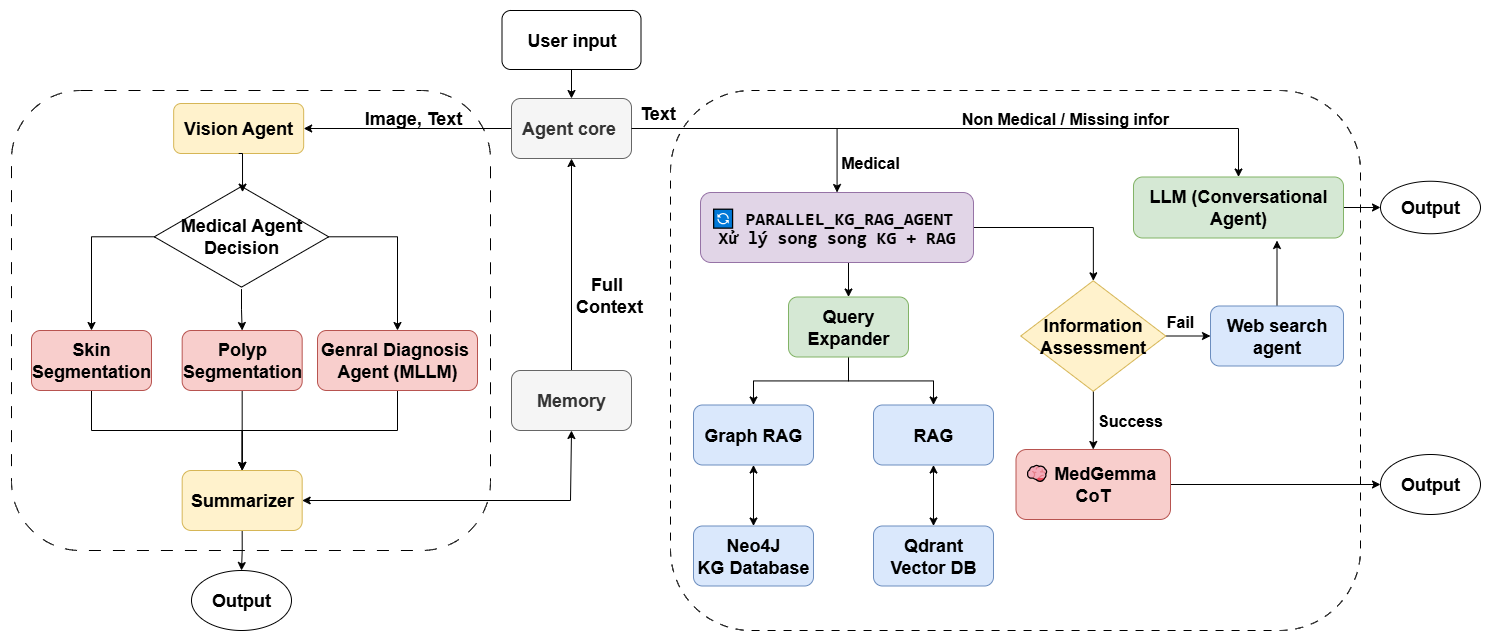
\includegraphics[width=1.0\textwidth]{images/chi_tiet.png}
    \caption{Kiến trúc chi tiết và luồng xử lý của hệ thống}
    \label{fig:detailed-architecture}
\end{figure}

Kiến trúc chi tiết của hệ thống Multi-Agent Medical Assistant được thiết kế theo mô hình modular với hai luồng xử lý chính được tách biệt rõ ràng: Vision Module và Text Module. Kiến trúc này đảm bảo khả năng xử lý hiệu quả các loại đầu vào khác nhau và tối ưu hóa hiệu suất cho từng loại tác vụ cụ thể.

\textbf{Agent Core (Bộ điều phối trung tâm):} Đây là thành phần trung tâm của hệ thống, có nhiệm vụ tiếp nhận đầu vào từ người dùng và thực hiện phân tích sơ bộ để xác định loại xử lý cần thiết. Agent Core sử dụng thuật toán phân loại thông minh để quyết định định tuyến yêu cầu đến Vision Module (cho xử lý hình ảnh và văn bản kèm theo) hoặc Text Module (cho xử lý thuần văn bản).

\textbf{Memory Management (Quản lý Bộ nhớ):} Hệ thống tích hợp một cơ chế quản lý bộ nhớ thông minh cho phép duy trì ngữ cảnh cuộc hội thoại và chia sẻ thông tin giữa các module. Bộ nhớ này lưu trữ lịch sử tương tác, kết quả phân tích trung gian, và thông tin bệnh nhân để đảm bảo tính liên tục và cá nhân hóa trong quá trình tư vấn.

\textbf{Full Context Integration:} Một tính năng quan trọng của kiến trúc là khả năng tích hợp toàn bộ ngữ cảnh từ cả hai module. Vision Module có thể cung cấp kết quả phân tích hình ảnh cho Text Module để hỗ trợ trong việc đưa ra chẩn đoán tổng hợp, trong khi Text Module có thể yêu cầu thông tin bổ sung từ Vision Module khi cần thiết.

\textbf{Parallel Processing Architecture:} Text Module được thiết kế với khả năng xử lý song song thông qua Parallel KG-RAG Agent, cho phép truy xuất thông tin đồng thời từ Knowledge Graph (Neo4j) và RAG Database (Qdrant). Kiến trúc này đảm bảo tốc độ phản hồi nhanh và độ bao phủ thông tin cao.

\textbf{MedGemma Chain of Thought:} Một điểm nổi bật trong kiến trúc mới là việc tích hợp MedGemma CoT (Chain of Thought), cho phép hệ thống thực hiện suy luận y khoa có cấu trúc và minh bạch. Cơ chế này đặc biệt quan trọng trong việc đảm bảo tính chính xác và khả năng giải thích của các quyết định y tế.

\subsubsection{Luồng hoạt động của tư vấn \& trả lời}

Luồng hoạt động của hệ thống Multi-Agent Medical Assistant được thiết kế theo một quy trình có tổ chức và thông minh, đảm bảo mỗi yêu cầu của người dùng được xử lý một cách chính xác và hiệu quả. Quá trình này được quản lý bởi LangGraph với khả năng duy trì trạng thái và điều phối các tác nhân chuyên biệt:

\begin{enumerate}
    \item \textbf{Phân tích và Tiền xử lý Đầu vào:} Hệ thống bắt đầu bằng việc phân tích đầu vào từ người dùng để xác định loại yêu cầu và tài nguyên cần thiết. Nếu có hình ảnh đi kèm, Vision Module sẽ thực hiện phân loại sơ bộ để xác định loại ảnh y tế (da liễu, nội soi, X-quang, v.v.). Đồng thời, hệ thống trích xuất và chuẩn hóa thông tin văn bản, chuẩn bị cho bước định tuyến tiếp theo.

    \item \textbf{Định tuyến Thông minh (Intelligent Routing):} Decision Agent sử dụng mô hình ngôn ngữ lớn để phân tích ngữ cảnh và nội dung yêu cầu, sau đó đưa ra quyết định định tuyến dựa trên các tiêu chí sau:
    \begin{itemize}
        \item \textit{Đối với câu hỏi y tế mơ hồ:} Định tuyến đến Conversation Agent để thu thập thêm thông tin thông qua multi-hop QA
        \item \textit{Đối với câu hỏi y tế cụ thể:} Định tuyến đến Parallel KG-RAG Agent để truy xuất thông tin chuyên môn
        \item \textit{Đối với yêu cầu phân tích hình ảnh:} Định tuyến đến các Vision Agent chuyên biệt (Skin Lesion, Polyp Segmentation, hoặc General Medical Image)
        \item \textit{Đối với thông tin y tế mới nhất:} Định tuyến đến Web Search Processor Agent
    \end{itemize}

    \item \textbf{Xử lý Song song và Tích hợp Nguồn:} Khi được định tuyến đến Parallel KG-RAG Agent, hệ thống thực hiện truy xuất thông tin đồng thời từ hai nguồn:
    \begin{itemize}
        \item \textit{Knowledge Graph (VietMedKG):} Sử dụng truy vấn Cypher để tìm kiếm thông tin có cấu trúc và mối quan hệ logic
        \item \textit{RAG Database (VimedAQA):} Thực hiện tìm kiếm vector ngữ nghĩa trong cơ sở dữ liệu tài liệu y khoa
    \end{itemize}
    Hệ thống đánh giá độ tin cậy của từng nguồn và quyết định chiến lược kết hợp hoặc fallback sang Web Search nếu cần thiết.

    \item \textbf{Multi-hop Question Answering (Hỏi đáp Đa bước):} Đối với các trường hợp thiếu thông tin lâm sàng, Conversation Agent kích hoạt cơ chế multi-hop QA:
    \begin{itemize}
        \item Thu thập thông tin về thời gian xuất hiện triệu chứng, mức độ nghiêm trọng, vị trí cụ thể
        \item Hỏi về các triệu chứng kèm theo, tiền sử bệnh lý, và thuốc đang sử dụng
        \item Đánh giá tính đầy đủ của thông tin trước khi chuyển sang bước chẩn đoán gợi ý
        \item Duy trì ngữ cảnh cuộc hội thoại và tránh hỏi lại các thông tin đã có
    \end{itemize}

    \item \textbf{Tổng hợp và Sinh Phản hồi:} Sau khi thu thập đủ thông tin, hệ thống sử dụng MedGemma 27B hoặc Gemini 2.0 Flash để:
    \begin{itemize}
        \item Tổng hợp thông tin từ các nguồn khác nhau
        \item Sinh ra phản hồi có cấu trúc với chẩn đoán gợi ý, khuyến nghị theo dõi, và trích dẫn nguồn
        \item Đánh giá mức độ rủi ro và xác định nhu cầu xác nhận từ con người
    \end{itemize}
    
    \item \textbf{Kiểm soát Chất lượng và An toàn (Guardrails):} Trước khi trả kết quả cho người dùng, hệ thống thực hiện:
    \begin{itemize}
        \item Kiểm tra nội dung có chứa thông tin có thể gây hại không
        \item Thêm các tuyên bố miễn trừ trách nhiệm và khuyến nghị khám bác sĩ khi cần
        \item Đánh giá nhu cầu xác nhận từ chuyên gia y tế (human-in-the-loop)
        \item Ghi log và theo dõi các phản hồi có độ rủi ro cao
    \end{itemize}

    \item \textbf{Phản hồi Cuối cùng và Theo dõi:} Hệ thống trình bày kết quả cho người dùng với:
    \begin{itemize}
        \item Thông tin chẩn đoán gợi ý có cấu trúc và dễ hiểu
        \item Khuyến nghị theo dõi và các bước tiếp theo
        \item Trích dẫn nguồn thông tin để người dùng có thể kiểm chứng
        \item Lưu trữ ngữ cảnh cuộc hội thoại cho các tương tác tiếp theo
    \end{itemize}
\end{enumerate}

Toàn bộ quy trình này được quản lý bởi LangGraph với khả năng duy trì trạng thái (StateGraph), cho phép hệ thống xử lý các luồng công việc phức tạp, quản lý ngoại lệ, và đảm bảo tính nhất quán trong toàn bộ quá trình tương tác với người dùng.

\subsection{Decision Agent}

Decision Agent đóng vai trò là bộ điều phối trung tâm, sử dụng LangGraph để điều phối các tác tử chuyên biệt. Chức năng chính của nó là phân tích yêu cầu của người dùng và định tuyến yêu cầu đó tới tác tử thích hợp nhất để xử lý. Điều này đảm bảo rằng mỗi yêu cầu được xử lý bởi thành phần có chuyên môn cao nhất, tối ưu hóa hiệu suất và độ chính xác của hệ thống.

\subsection{Vision Module}

\begin{figure}[H]
    \centering
    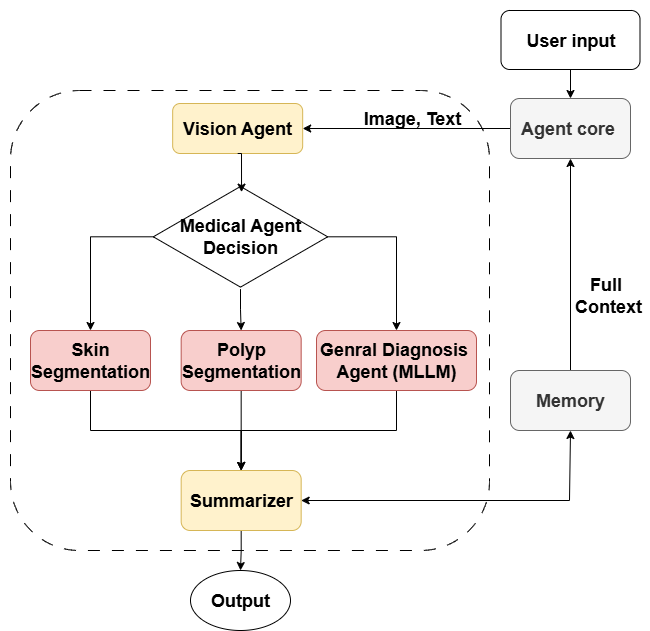
\includegraphics[width=0.8\textwidth]{images/vision.png}
    \caption{Kiến trúc chi tiết của Vision Module với luồng xử lý hình ảnh y tế}
    \label{fig:vision-module}
\end{figure}

Vision Module trong hệ thống Multi-Agent Medical Assistant được thiết kế như một hệ thống xử lý hình ảnh y tế chuyên biệt với kiến trúc modular và khả năng mở rộng cao. Module này đảm nhận vai trò quan trọng trong việc phân tích, chẩn đoán và tư vấn dựa trên thông tin hình ảnh y tế.

\textbf{Agent Core Integration:} Vision Module nhận đầu vào từ Agent Core dưới dạng kết hợp giữa hình ảnh và văn bản mô tả. Quá trình tích hợp này cho phép hệ thống hiểu được ngữ cảnh của hình ảnh thông qua thông tin văn bản kèm theo, từ đó cung cấp phân tích chính xác và phù hợp hơn.

\textbf{Medical Agent Decision (Bộ Phân loại Hình ảnh Y tế):} Đây là thành phần trí tuệ nhân tạo đầu tiên trong Vision Module, có nhiệm vụ phân loại loại hình ảnh y tế được tải lên. Hệ thống sử dụng các mô hình machine learning tiên tiến để nhận diện và phân loại hình ảnh vào các danh mục chính:
\begin{itemize}
    \item Hình ảnh tổn thương da (dermatology images)
    \item Hình ảnh nội soi đại tràng với polyp
    \item Hình ảnh y tế tổng quát (X-quang, MRI, CT, siêu âm, v.v.)
\end{itemize}

\textbf{Specialized Processing Agents:} Dựa trên kết quả phân loại, hình ảnh được định tuyến đến một trong ba tác nhân chuyên biệt:

\textbf{Skin Segmentation Agent:} Tác nhân này chuyên xử lý hình ảnh tổn thương da sử dụng kiến trúc U-Net được fine-tuning trên các dataset dermatology chuyên biệt. Với khả năng học sâu từ hàng nghìn hình ảnh tổn thương da đã được chuyên gia da liễu gán nhãn, agent này có thể phân vùng chính xác ranh giới tổn thương da, tách biệt rõ ràng giữa vùng da bình thường và vùng da bị tổn thương. 

\textbf{Polyp Segmentation Agent:} Đây là tác nhân chuyên biệt dành riêng cho phân tích hình ảnh nội soi đại tràng, sử dụng kiến trúc DeepLabV3+ được tối ưu hóa cho việc phát hiện và phân vùng polyp. Agent này không chỉ có khả năng phát hiện và phân vùng polyp trong hình ảnh nội soi một cách chính xác mà còn có thể phân loại polyp theo mức độ nguy hiểm, phân biệt giữa polyp neoplastic (có khả năng ác tính) và non-neoplastic (lành tính). Khả năng phân loại này dựa trên các đặc điểm hình thái học được học từ cơ sở dữ liệu lớn các hình ảnh nội soi đã được chuyên gia tiêu hóa xác nhận.

\textbf{General Diagnosis Agent (MLLM):} Tác nhân này sử dụng mô hình ngôn ngữ đa phương thức lớn (Multimodal Large Language Model) để xử lý các loại hình ảnh y tế tổng quát không thuộc hai danh mục chuyên biệt trên. Với khả năng tích hợp tri thức y khoa rộng lớn, agent này có thể phân tích và mô tả chi tiết các đặc điểm bất thường trong hình ảnh, từ X-quang, MRI, CT scan đến siêu âm và các loại hình ảnh y tế khác. Ngoài việc mô tả các findings, agent còn có khả năng đưa ra chẩn đoán sơ bộ dựa trên tri thức y khoa đã được học và cung cấp khuyến nghị về các xét nghiệm hoặc thăm khám bổ sung cần thiết.

\textbf{Intelligent Summarizer:} Tất cả kết quả từ các tác nhân chuyên biệt được tập hợp tại Summarizer - một thành phần AI thông minh có nhiệm vụ:
Tổng hợp và tích hợp kết quả phân tích từ các agent chuyên biệt
    Sinh ra báo cáo có cấu trúc với ngôn ngữ dễ hiểu cho người dùng phổ thông
    Đưa ra khuyến nghị theo dõi và các bước tiếp theo cần thực hiện
    Đánh giá mức độ cấp thiết và cần thiết phải thăm khám y tế

\subsection{Advanced Post-Processing Technique}

Một đóng góp quan trọng trong Polyp Segmentation Agent là việc phát triển kỹ thuật hậu xử lý tiên tiến nhằm cải thiện độ chính xác của quá trình phân vùng. Kỹ thuật này sử dụng phân tích thành phần liên thông (Connected Component Analysis) kết hợp với kiểm tra sự thống trị màu sắc ở mức pixel để tăng cường tính nhất quán trong từng vùng được phân đoạn.

\subsubsection{Phương pháp tiếp cận}

Quy trình bao gồm hai bước chính: đầu tiên, hệ thống sử dụng hàm ndimage.label để xác định các thành phần liên thông trong mask phân vùng, tách các vùng không phải nền thành các khu vực riêng biệt dựa trên tính liên thông trong đồ thị pixel. Tiếp theo, đối với các vùng đơn sắc (chỉ chứa một lớp), hệ thống giữ nguyên không thay đổi. Đối với các vùng đa sắc (chứa nhiều lớp), hệ thống xác định lớp thống trị bằng cách đếm số pixel của từng lớp, sau đó điền toàn bộ vùng với màu tương ứng với lớp thống trị.

\subsubsection{Kết quả cải thiện}

Kỹ thuật này đã được kiểm chứng trên dataset BKAI IGH NeoPolyp-Small với độ phân giải chuẩn hóa 512x512, cho thấy cải thiện đáng kể về độ chính xác Dice Score khoảng 3-4\% trên các mô hình khác nhau. Đặc biệt, mô hình DeepLabV3+ với backbone RegNetx320 đạt được kết quả tốt nhất với Dice Score 86.33\% sau khi áp dụng post-processing, so với 82.56\% khi không sử dụng kỹ thuật này. Sự cải thiện này chứng minh hiệu quả của việc loại bỏ nhiễu và tăng cường tính nhất quán trong các vùng phân đoạn, đặc biệt quan trọng trong ứng dụng lâm sàng nơi độ chính xác phân vùng là yếu tố then chốt.

\subsection{Text Module}

\begin{figure}[H]
    \centering
    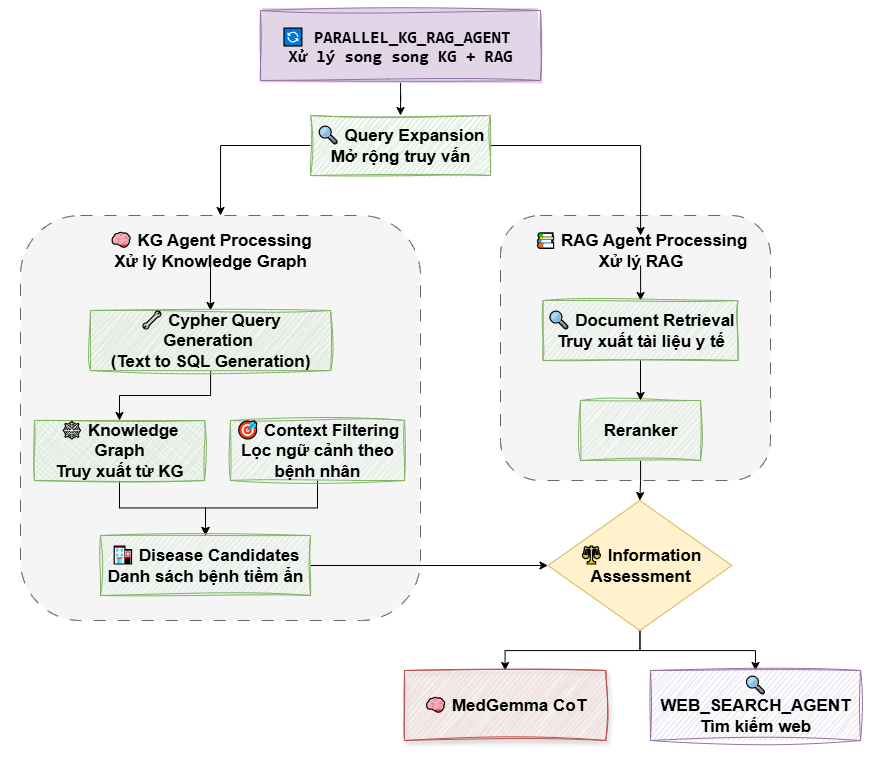
\includegraphics[width=0.75\textwidth]{images/text_module.png}
    \caption{Kiến trúc chi tiết của Text Module với xử lý song song KG-RAG}
    \label{fig:text-module}
\end{figure}

\begin{figure}[H]
    \centering
    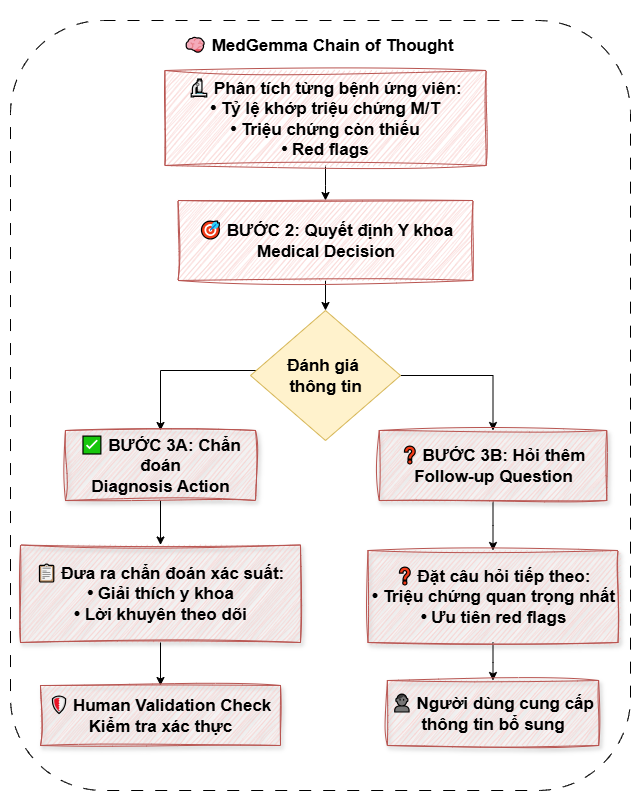
\includegraphics[width=0.45\textwidth]{images/medcot.png}
    \caption{MedGemma Chain of Thought - Quy trình suy luận y khoa có cấu trúc}
    \label{fig:medcot}
\end{figure}


Text Module trong hệ thống Multi-Agent Medical Assistant được thiết kế như một hệ thống xử lý ngôn ngữ tự nhiên chuyên biệt cho lĩnh vực y tế, với khả năng tích hợp đa nguồn thông tin và suy luận thông minh. Module này đóng vai trò trung tâm trong việc xử lý các truy vấn văn bản, từ câu hỏi y tế đơn giản đến các tình huống lâm sàng phức tạp yêu cầu suy luận đa bước.

\subsubsection{Knowledge Graph Agent (KG Agent)}

Knowledge Graph Agent là thành phần chuyên biệt cho việc truy xuất thông tin có cấu trúc từ VietMedKG thông qua các truy vấn Cypher phức tạp. Agent này được thiết kế để khai thác tối đa các mối quan hệ logic giữa các thực thể y tế và cung cấp thông tin có độ chính xác cao dựa trên tri thức y khoa có cấu trúc.

\textbf{Cypher Query Service:} Thành phần cốt lõi của KG Agent, có nhiệm vụ chuyển đổi câu hỏi ngôn ngữ tự nhiên thành các truy vấn Cypher để tương tác với Neo4j database. Hệ thống sử dụng GraphCypherQAChain với few-shot learning, cho phép mô hình học từ các ví dụ truy vấn mẫu để sinh ra các câu lệnh Cypher chính xác. Quá trình này được hỗ trợ bởi Gemini 2.0 Flash với temperature=0.0 để đảm bảo tính nhất quán và chính xác trong việc sinh truy vấn.

\textbf{Context Filtering với Embedding:} Sau khi truy xuất thông tin từ Knowledge Graph, hệ thống áp dụng cơ chế lọc ngữ cảnh thông minh sử dụng embedding similarity. ContextFilterEmbedding sử dụng FPT Vietnamese Embedding để tính toán độ tương đồng cosine giữa truy vấn và các ứng viên bệnh từ KG. Hệ thống không chỉ xem xét điểm tương đồng mà còn phân tích số lượng triệu chứng khớp (matched\_symptoms) và tổng số triệu chứng (total\_symptoms) để đưa ra quyết định lọc thông minh.

\textbf{Patient-Specific Context Integration:} Một tính năng quan trọng của KG Agent là khả năng tích hợp thông tin bệnh nhân cụ thể vào quá trình truy vấn. Hệ thống sử dụng QueryExpander để tinh chỉnh truy vấn dựa trên hồ sơ bệnh nhân (tuổi, giới tính, tiền sử bệnh, bệnh hiện tại) và lịch sử hội thoại, đảm bảo kết quả truy xuất có tính cá nhân hóa cao.

\subsubsection{RAG Agent (Retrieval-Augmented Generation Agent)}

RAG Agent chuyên trách việc truy xuất và xử lý thông tin từ cơ sở dữ liệu tài liệu y khoa VimedAQA được lưu trữ trong Qdrant Vector Database. Agent này sử dụng các kỹ thuật tìm kiếm vector hiện đại kết hợp với reranking để đảm bảo chất lượng thông tin truy xuất cao nhất.

\textbf{Vector Store Management:} RAG Agent sử dụng VectorStoreCloud để quản lý việc lưu trữ và truy xuất documents trong Qdrant. Hệ thống hỗ trợ cả dense vector search với E5 Multilingual Large Instruct embedding model, cho phép tìm kiếm ngữ nghĩa chính xác trên corpus tiếng Việt. Vector store được tối ưu hóa với distance metric COSINE và indexing threshold = 0 để đảm bảo tốc độ truy vấn nhanh nhất.

\textbf{Query Expansion và Preprocessing:} Trước khi thực hiện tìm kiếm, RAG Agent sử dụng QueryExpander để mở rộng truy vấn bằng cách bổ sung các thuật ngữ y khoa liên quan, từ đồng nghĩa, và các biến thể ngôn ngữ. Quá trình này được thực hiện bởi LLM với prompt engineering chuyên biệt, đảm bảo không bỏ sót thông tin quan trọng trong quá trình tìm kiếm.

\textbf{Hybrid Search và Document Retrieval:} RAG Agent thực hiện tìm kiếm kết hợp (hybrid search) tích hợp cả similarity search dựa trên vector embeddings và keyword matching. Hệ thống truy xuất top-k documents có độ liên quan cao nhất từ Qdrant, với mỗi document được gán score dựa trên độ tương đồng cosine. Quá trình này được tối ưu hóa để xử lý cả short queries và long-form medical descriptions.

\textbf{Advanced Reranking:} Sau khi truy xuất, các documents được xử lý qua Reranker sử dụng CrossEncoder model (pritamdeka/S-PubMedBert-MS-MARCO) được fine-tuning cho domain y tế. Reranker tính toán combined\_score bằng cách kết hợp original similarity score và rerank\_score, sau đó sắp xếp lại documents theo thứ tự độ liên quan thực tế cao nhất.

\textbf{Response Generation với Medical Chain of Thought:} RAG Agent sử dụng ResponseGenerator với medical-specific prompting để sinh phản hồi có cấu trúc. Hệ thống áp dụng chain of thought reasoning gồm 3 bước: (1) Phân tích tài liệu và đối chiếu, (2) Quyết định y khoa (ENOUGH\_INFO/NOT\_ENOUGH\_INFO), (3) Hành động phù hợp. Mọi phản hồi đều được kèm theo safety disclaimer và source citations để đảm bảo tính minh bạch và an toàn.

\subsubsection{MedGemma Chain of Thought}

MedGemma Chain of Thought là một đột phá quan trọng trong việc áp dụng suy luận y khoa có cấu trúc vào hệ thống AI. Cơ chế này mô phỏng quy trình tư duy của các chuyên gia y tế, đảm bảo tính logic và minh bạch trong mọi quyết định chẩn đoán.

\textbf{Bước 1 - Phân tích Từng Bệnh Ứng viên:} Hệ thống bắt đầu bằng việc phân tích chi tiết các triệu chứng và thông tin lâm sàng được cung cấp. MedGemma 27B sử dụng tri thức y khoa chuyên sâu để xác định các red flags (dấu hiệu cảnh báo) và đánh giá mức độ khẩn cấp của tình trạng bệnh nhân.

\textbf{Bước 2 - Quyết định Y khoa (Medical Decision):} Dựa trên phân tích ở bước 1, hệ thống đưa ra quyết định về hướng xử lý tiếp theo. Đây là bước quan trọng nhất trong quy trình, yêu cầu sự cân nhắc kỹ lưỡng giữa các yếu tố lâm sàng và mức độ rủi ro.

\textbf{Bước 3 - Đánh giá Thông tin và Phân nhánh:} Hệ thống đánh giá tính đầy đủ của thông tin hiện có và quyết định một trong hai hướng xử lý. Nếu thông tin đủ để đưa ra chẩn đoán gợi ý (Bước 3A), hệ thống sẽ tiến hành tổng hợp kết quả và đưa ra khuyến nghị. Nếu thông tin chưa đầy đủ (Bước 3B), hệ thống sẽ kích hoạt cơ chế Multi-hop QA để thu thập thêm thông tin cần thiết.

\textbf{Multi-hop Question Answering:} Khi được kích hoạt, cơ chế này thực hiện một chuỗi câu hỏi có cấu trúc để thu thập đầy đủ thông tin lâm sàng. Hệ thống đặt các câu hỏi về triệu chứng quan trọng nhất, ưu tiên các red flags, và dần dần thu thập thông tin chi tiết về thời gian, mức độ, vị trí, và các yếu tố liên quan. Quá trình này tiếp tục cho đến khi có đủ thông tin để đưa ra quyết định y khoa tin cậy.

\textbf{Human Validation Check:} Trước khi đưa ra phản hồi cuối cùng, hệ thống thực hiện kiểm tra xác thực con người (Human Validation Check) cho các trường hợp có độ rủi ro cao hoặc yêu cầu can thiệp y tế khẩn cấp. Cơ chế này đảm bảo an toàn tối đa cho người dùng và tuân thủ các nguyên tắc y đức.

\subsubsection{Web Search Agent}

Web Search Agent đóng vai trò như một cầu nối quan trọng giữa tri thức nội bộ của hệ thống và thông tin y tế mới nhất trên internet. Agent này được kích hoạt trong hai tình huống chính: khi kết quả từ Parallel KG-RAG Agent có độ tin cậy thấp, hoặc khi cần truy xuất thông tin về các phát triển y tế gần đây mà cơ sở dữ liệu nội bộ chưa cập nhật.

Hệ thống thực hiện tìm kiếm thông minh trên các nguồn đáng tin cậy như Tavily, PubMed, và các trang web y khoa uy tín khác. Quá trình tìm kiếm được tối ưu hóa với các từ khóa y khoa chuyên biệt và được lọc theo độ uy tín của nguồn. Chức năng chính của Web Search Agent là tổng hợp và cập nhật thông tin mới nhất từ internet, bổ sung vào kho kiến thức của hệ thống để đảm bảo các phản hồi luôn được cập nhật, chính xác và phù hợp với thực tiễn y tế mới nhất.

\subsubsection{Conversational Agent}

Conversational Agent chịu trách nhiệm xử lý các cuộc hội thoại tự nhiên giữa người dùng và hệ thống, đặc biệt quan trọng trong việc triển khai cơ chế Multi-hop QA. Agent này không chỉ tập trung vào các tương tác đơn giản như hỏi đáp và trò chuyện, mà còn đóng vai trò quan trọng trong việc dẫn dắt cuộc hội thoại theo hướng thu thập thông tin lâm sàng có cấu trúc.

Khi được kích hoạt bởi MedGemma Chain of Thought, Conversational Agent sử dụng các kỹ thuật hỏi đáp thông minh để thu thập từng phần thông tin cần thiết một cách tự nhiên và không gây áp lực cho người dùng. Agent này được trang bị khả năng duy trì ngữ cảnh cuộc hội thoại, tránh hỏi lại các thông tin đã có, và điều chỉnh phong cách giao tiếp phù hợp với từng đối tượng người dùng khác nhau.

\subsection{Patient Database Agent - Hệ thống Theo dõi Sức khỏe}

Patient Database Agent là một thành phần quan trọng của hệ thống, chuyên trách quản lý thông tin bệnh nhân và theo dõi các chỉ số sức khỏe theo thời gian. Agent này không chỉ lưu trữ dữ liệu mà còn có khả năng phân tích xu hướng, phát hiện bất thường và tạo ra các báo cáo y tế chuyên nghiệp.

\begin{figure}[H]
    \centering
    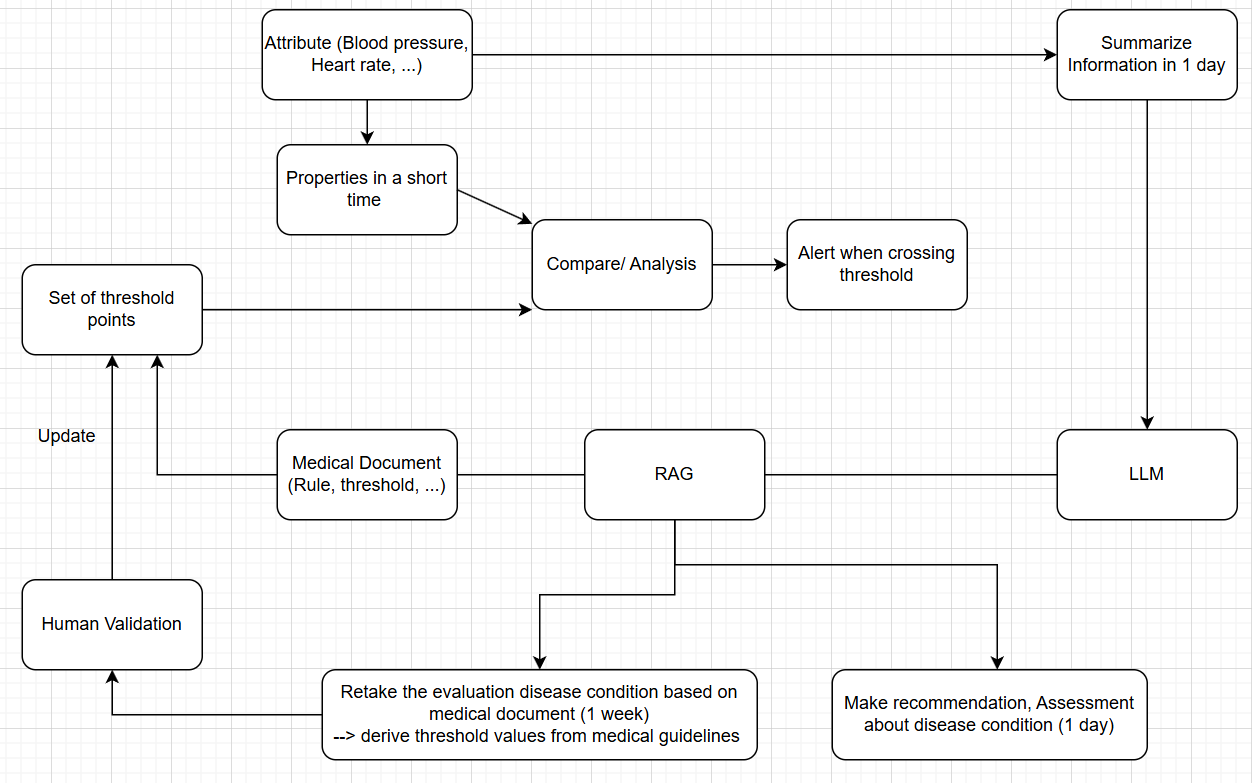
\includegraphics[width=1.0\textwidth]{images/blood_pressure_system.png}
    \caption{Kiến trúc hệ thống theo dõi chỉ số sức khỏe thông minh}
    \label{fig:blood-pressure-system}
\end{figure}

\subsubsection{Kiến trúc Hệ thống Theo dõi Thông minh}

Hệ thống theo dõi sức khỏe được thiết kế theo mô hình phân tích thông minh với khả năng học hỏi và thích ứng theo từng bệnh nhân cụ thể. Kiến trúc bao gồm các thành phần chính:

\textbf{Thu thập Dữ liệu Đa nguồn:} Hệ thống có khả năng thu thập thông tin sức khỏe từ nhiều nguồn khác nhau, bao gồm nhập liệu thủ công qua form điện tử, kết nối với các thiết bị đo y tế (máy đo huyết áp, máy đo đường huyết, cân thông minh), và tích hợp dữ liệu từ các ứng dụng sức khỏe khác. Mỗi loại dữ liệu được chuẩn hóa và xác thực trước khi lưu trữ.

\textbf{Xử lý Thời gian Thực:} Agent thực hiện phân tích dữ liệu ngay khi nhận được, tính toán các chỉ số thống kê cơ bản như giá trị trung bình, độ biến thiên, và xu hướng trong ngắn hạn. Hệ thống có khả năng phát hiện các giá trị bất thường và cảnh báo ngay lập tức khi các chỉ số vượt quá ngưỡng an toàn.

\textbf{Hệ thống Ngưỡng Thông minh:} Một trong những đặc điểm nổi bật của hệ thống là khả năng thiết lập và điều chỉnh ngưỡng cảnh báo một cách thông minh. Thay vì sử dụng các ngưỡng cố định, hệ thống sử dụng kết hợp giữa guidelines y khoa chuẩn và dữ liệu cá nhân của bệnh nhân để tạo ra các ngưỡng được cá nhân hóa. Quá trình này được hỗ trợ bởi RAG Agent để truy xuất thông tin từ tài liệu y khoa và được xác thực bởi chuyên gia y tế thông qua cơ chế Human Validation.

\subsubsection{Quy trình Phân tích và Cảnh báo}

Hệ thống hoạt động theo một quy trình có cấu trúc, đảm bảo tính chính xác và kịp thời trong việc phát hiện các vấn đề sức khỏe:

\textbf{Bước 1 - Thu thập và Chuẩn hóa:} Dữ liệu từ các nguồn khác nhau được thu thập và chuẩn hóa theo format thống nhất. Hệ thống thực hiện kiểm tra tính hợp lệ của dữ liệu, loại bỏ các giá trị nhiễu và bổ sung metadata cần thiết như thời gian đo, điều kiện đo (trước/sau ăn, nghỉ ngơi/hoạt động).

\textbf{Bước 2 - Phân tích Ngắn hạn:} Trong khoảng thời gian ngắn (vài giờ đến 1 ngày), hệ thống tính toán các chỉ số thống kê cơ bản và so sánh với ngưỡng đã thiết lập. Nếu phát hiện bất thường, hệ thống sẽ kích hoạt cảnh báo tức thì và gửi thông báo cho người dùng.

\textbf{Bước 3 - So sánh và Phân tích:} Dữ liệu mới được so sánh với lịch sử của bệnh nhân và các ngưỡng cá nhân hóa. Hệ thống sử dụng các thuật toán machine learning đơn giản để phát hiện các pattern bất thường và xu hướng đáng lo ngại.

\textbf{Bước 4 - Tạo Báo cáo Thông minh:} Định kỳ (hàng ngày, hàng tuần), hệ thống tự động tổng hợp dữ liệu và tạo ra các báo cáo phân tích chuyên sâu. Quá trình này được hỗ trợ bởi LLM để tạo ra các báo cáo dễ hiểu, có cấu trúc và chứa các khuyến nghị cụ thể.

\subsubsection{Tích hợp RAG và Cập nhật Ngưỡng}

Một đặc điểm độc đáo của hệ thống là khả năng tự cập nhật và cải thiện các ngưỡng cảnh báo dựa trên tài liệu y khoa mới nhất:

\textbf{Truy xuất Tài liệu Y khoa:} RAG Agent được kích hoạt định kỳ để tìm kiếm các guidelines y khoa mới nhất, nghiên cứu lâm sàng và khuyến nghị từ các tổ chức y tế uy tín. Thông tin này được sử dụng để đánh giá lại tính phù hợp của các ngưỡng hiện tại.

\textbf{Đánh giá Lại Điều kiện Bệnh:} Hệ thống thực hiện đánh giá lại tình trạng sức khỏe của bệnh nhân sau mỗi tuần, dựa trên dữ liệu thu thập được và thông tin y khoa mới. Quá trình này giúp xác định liệu các ngưỡng cảnh báo có cần điều chỉnh hay không.

\textbf{Cơ chế Human Validation:} Mọi thay đổi quan trọng về ngưỡng cảnh báo hoặc đánh giá tình trạng bệnh đều phải được xác thực bởi chuyên gia y tế. Hệ thống tự động gửi yêu cầu xác nhận và chỉ áp dụng thay đổi sau khi được phê duyệt.

\subsubsection{Tính năng Báo cáo Y tế Tự động}

Patient Database Agent có khả năng tạo ra các loại báo cáo y tế khác nhau, phục vụ cho nhiều mục đích:

\textbf{Báo cáo Hàng ngày:} Tóm tắt các chỉ số quan trọng trong ngày, so sánh với ngày trước đó và đưa ra nhận xét về xu hướng. Báo cáo bao gồm biểu đồ trực quan và các khuyến nghị cụ thể cho ngày tiếp theo.

\textbf{Báo cáo Tuần/Tháng:} Phân tích xu hướng dài hạn, đánh giá hiệu quả của các can thiệp điều trị và đưa ra khuyến nghị về việc điều chỉnh phác đồ điều trị. Báo cáo này được thiết kế để hỗ trợ bác sĩ trong việc ra quyết định lâm sàng.

\textbf{Báo cáo Chuyên biệt:} Khi phát hiện các pattern bất thường hoặc có yêu cầu từ bác sĩ, hệ thống có thể tạo ra các báo cáo chuyên biệt tập trung vào một khía cạnh cụ thể của sức khỏe bệnh nhân.

\subsubsection{Ví dụ Ứng dụng: Theo dõi Huyết áp}

Để minh họa khả năng của hệ thống, chúng ta xem xét trường hợp theo dõi huyết áp:

Hệ thống thu thập dữ liệu huyết áp từ thiết bị đo tự động mỗi 30 giây trong 7 ngày liên tục. Với hơn 20.000 lần đo, hệ thống có thể phân tích chi tiết các pattern như biến thiên theo circadian rhythm, phản ứng với hoạt động thể chất, và hiệu quả của thuốc hạ áp.

RAG Agent được sử dụng để truy xuất guidelines mới nhất từ American Heart Association và European Society of Cardiology, giúp thiết lập các ngưỡng cảnh báo phù hợp với tình trạng cụ thể của bệnh nhân. LLM được sử dụng để tạo ra báo cáo phân tích chi tiết, bao gồm đánh giá nguy cơ tim mạch, khuyến nghị về điều chỉnh thuốc và lối sống.

Kết quả là một hệ thống theo dõi toàn diện, có khả năng phát hiện sớm các biến đổi bất thường và hỗ trợ bác sĩ trong việc đưa ra quyết định điều trị tối ưu.

\begin{figure}[H]
    \centering
    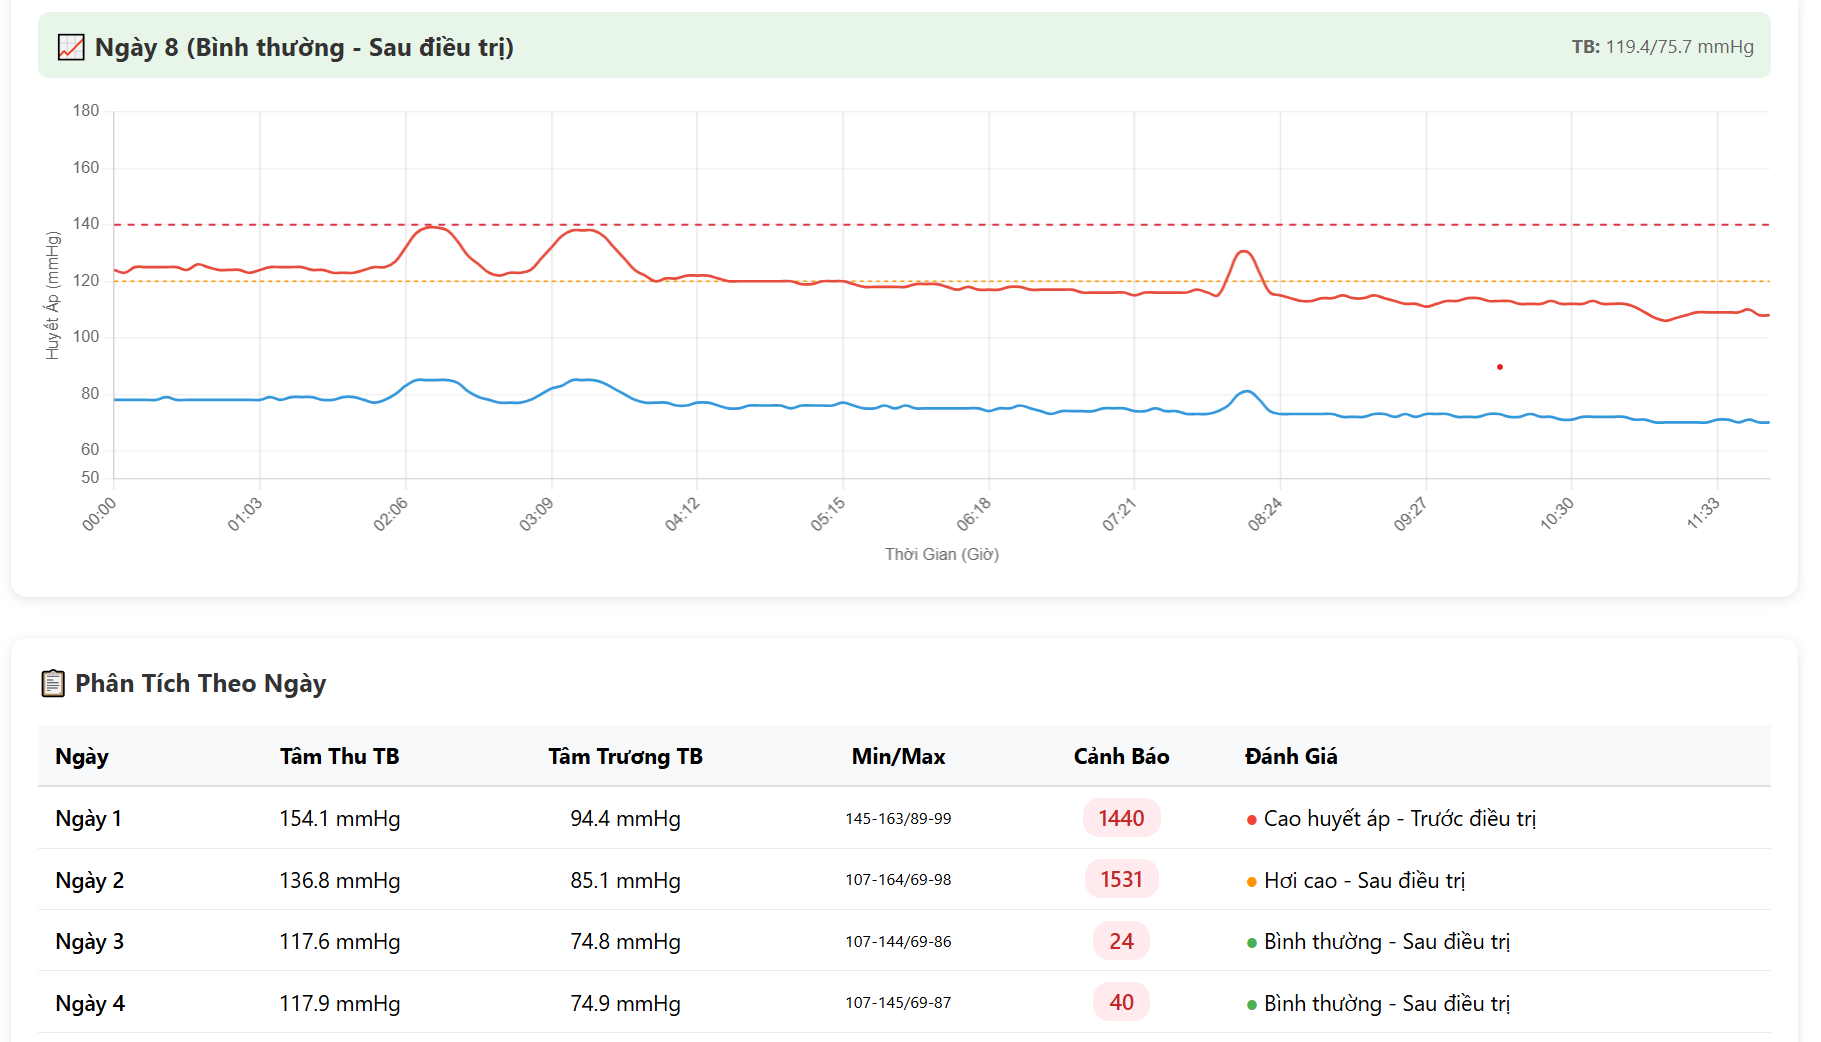
\includegraphics[width=1.0\textwidth]{images/blood_pressure_demo.png}
    \caption{Demo dữ liệu huyết áp bệnh nhân}
    \label{fig:demo-overview}
\end{figure}

\section{Dataset và Đánh giá kết quả}

\subsection{Dataset}

Hệ thống Multi-Agent Medical Assistant được xây dựng trên nền tảng dữ liệu y tế tiếng Việt toàn diện, bao gồm ba bộ dữ liệu chính được tích hợp một cách có hệ thống:

\textbf{VietMedKG (Vietnamese Medical Knowledge Graph):} Đây là cơ sở tri thức y khoa có cấu trúc được thiết kế đặc biệt cho ngữ cảnh y tế Việt Nam. VietMedKG chứa các mối quan hệ phức tạp giữa các thực thể y tế như bệnh tật, triệu chứng, thuốc men, phương pháp điều trị, và các yếu tố nguy cơ. Cấu trúc đồ thị này cho phép hệ thống thực hiện các truy vấn Cypher phức tạp để truy xuất thông tin có ngữ cảnh và mối liên hệ logic, hỗ trợ đặc biệt hiệu quả cho các câu hỏi y tế đa bước và suy luận chẩn đoán.

\begin{figure}[H]
    \centering
    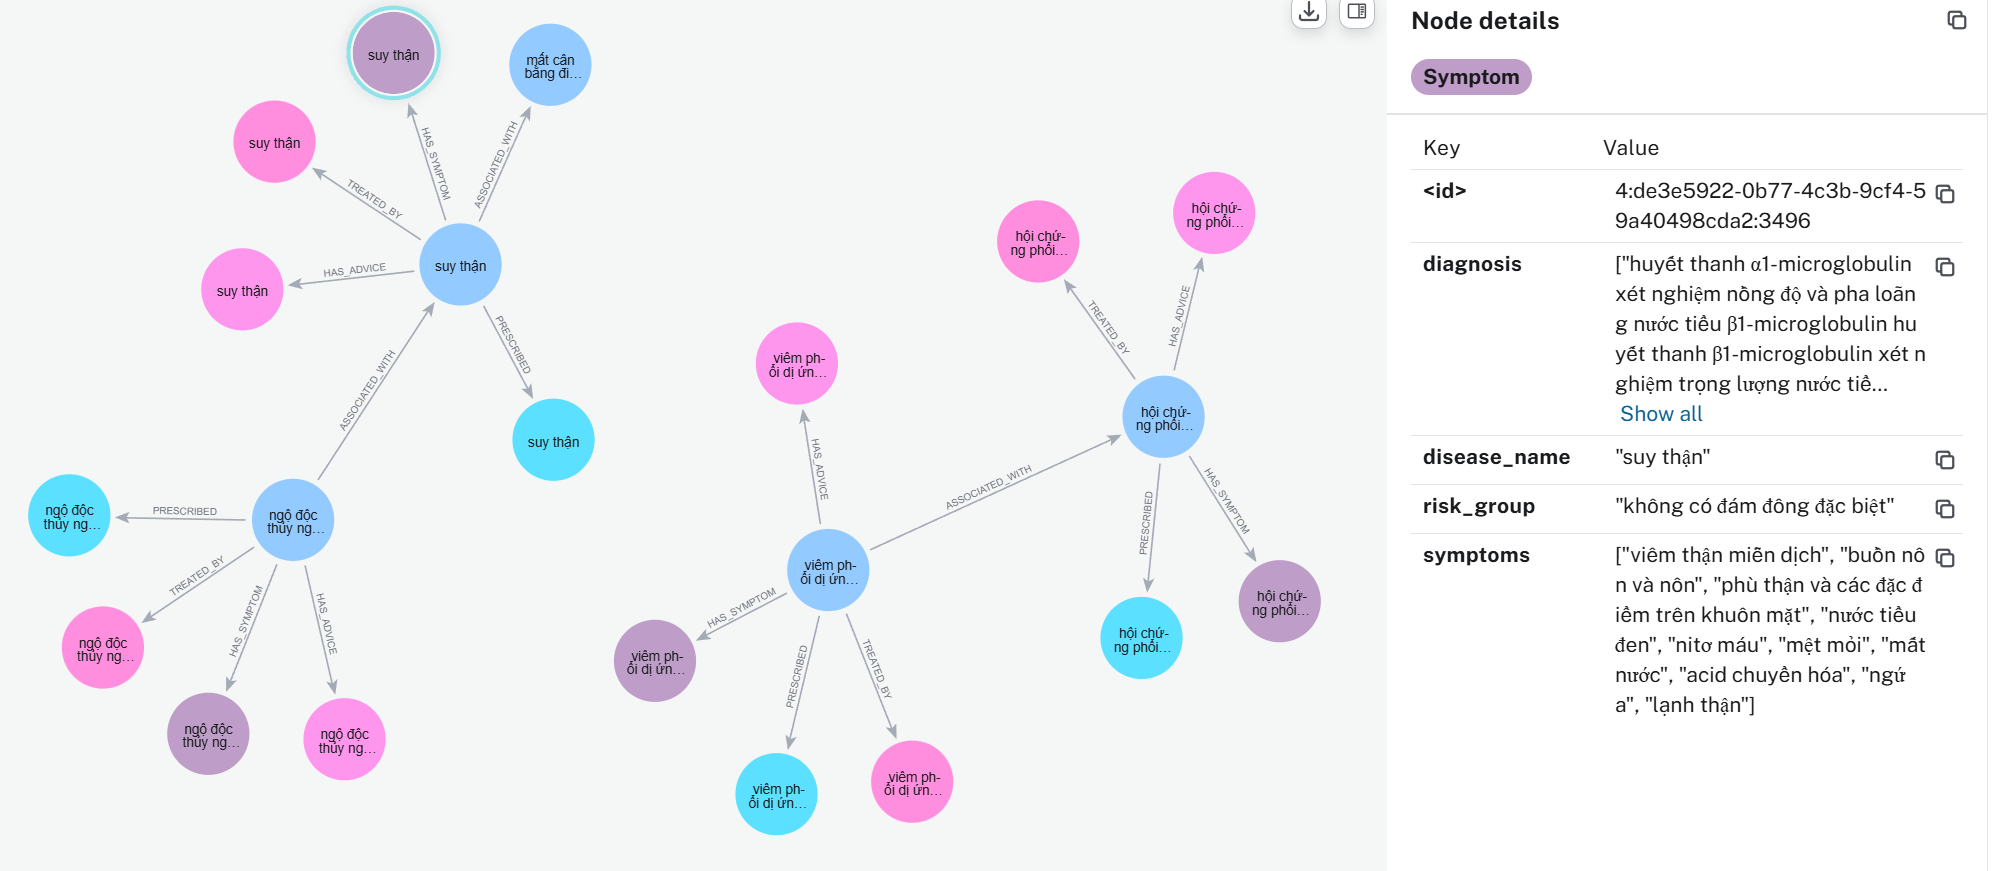
\includegraphics[width=1.0\textwidth]{images/KG database.png}
    \caption{Tổng quan bộ dữ liệu VietMedKG}
    \label{fig:dataset-kg-overview}
\end{figure}

\textbf{VimedAQA (Vietnamese Medical Question-Answer Dataset):} Bộ dữ liệu này cung cấp nền tảng cho tác nhân RAG với hàng nghìn cặp câu hỏi-trả lời y tế bằng tiếng Việt, bao gồm nhiều chuyên khoa như nội khoa, ngoại khoa, sản phụ khoa, nhi khoa, và y học cổ truyền. Dữ liệu được cấu trúc dưới dạng vector embeddings trong Qdrant, cho phép tìm kiếm ngữ nghĩa hiệu quả và truy xuất thông tin có độ liên quan cao với truy vấn của người dùng.

\begin{figure}[H]
    \centering
    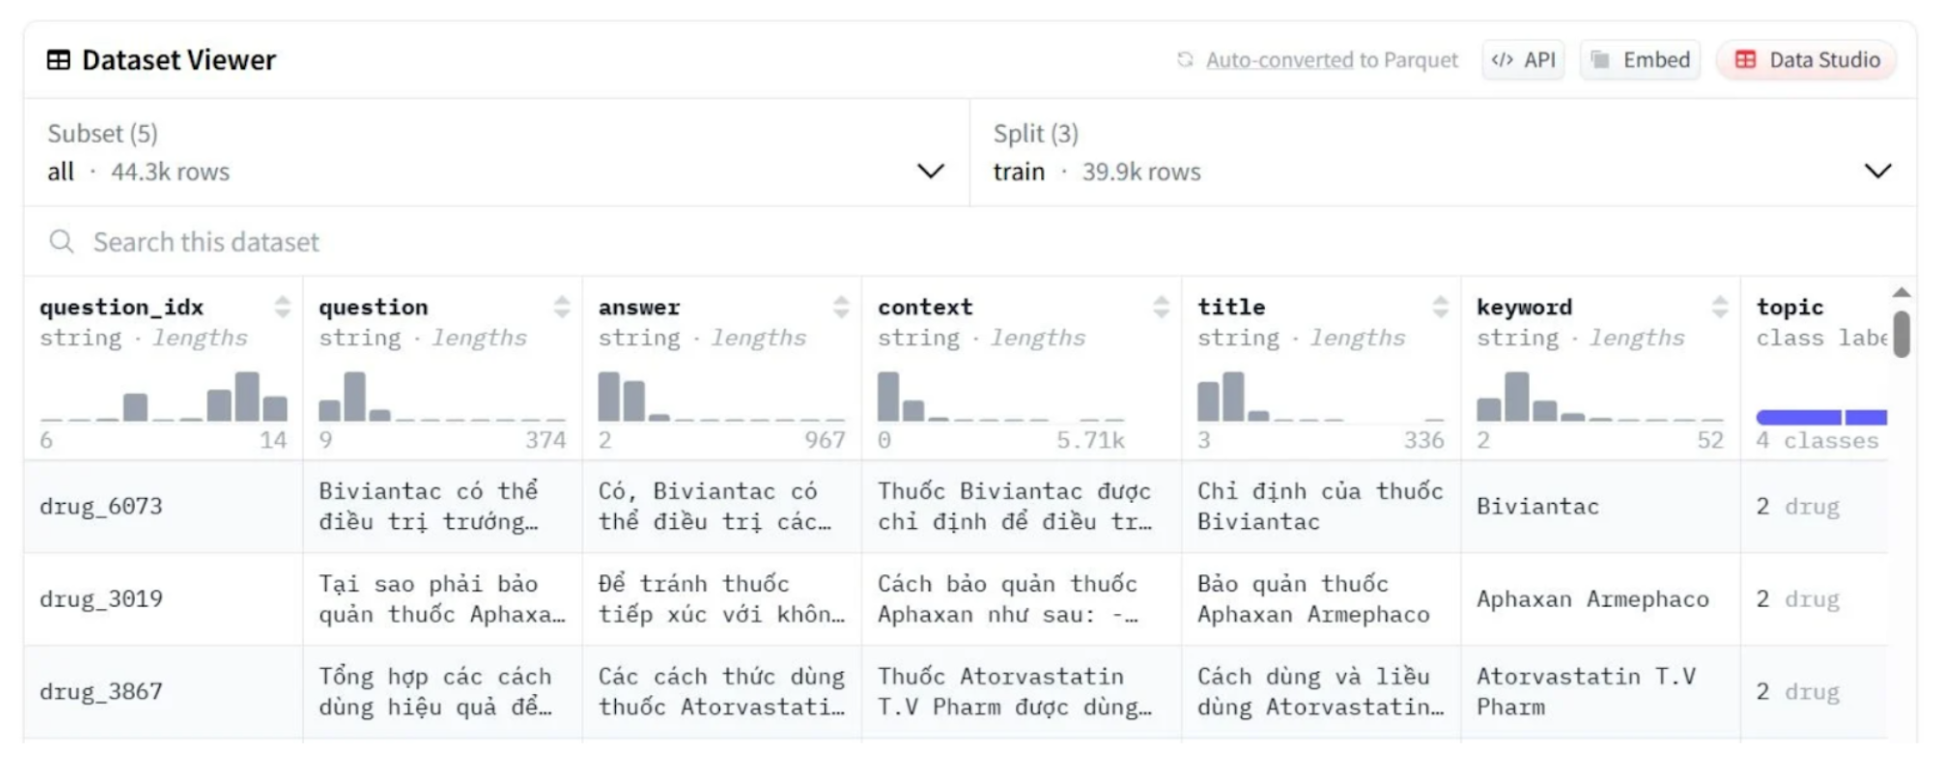
\includegraphics[width=1.0\textwidth]{images/image.png}
    \caption{Tổng quan bộ dữ liệu VimedAQA}
    \label{fig:dataset-overview}
\end{figure}

\textbf{BKAI-IGH NeoPolyp-Small Dataset:} Bộ dữ liệu chuyên biệt được phát triển bởi Lan và cộng sự cho bài toán phân đoạn polyp đại tràng và phát hiện tân sinh. Dataset bao gồm 1.200 hình ảnh nội soi đại tràng chất lượng cao với chú thích phân đoạn chi tiết, trong đó có 1.000 hình ảnh WLI (White Light Imaging) và 200 hình ảnh FICE (Flexible spectral Imaging Color Enhancement). Đặc biệt, tất cả polyp được phân loại thành hai nhóm quan trọng về mặt lâm sàng: neoplastic (có khả năng ác tính, được đánh dấu màu đỏ) và non-neoplastic (lành tính, được đánh dấu màu xanh lá). Dataset được chia thành tập huấn luyện 1.000 hình ảnh và tập kiểm tra 200 hình ảnh, với độ phân giải chuẩn hóa 512x512 pixel, tạo điều kiện thuận lợi cho việc đánh giá khách quan các mô hình phân đoạn polyp.

Việc kết hợp ba nguồn dữ liệu này tạo ra một hệ sinh thái thông tin y tế toàn diện: VietMedKG cung cấp tri thức có cấu trúc cho suy luận logic, VimedAQA cung cấp thông tin chi tiết cho các tình huống lâm sàng, và BKAI-IGH NeoPolyp-Small hỗ trợ phân tích hình ảnh y tế chuyên sâu, đặc biệt trong lĩnh vực nội soi tiêu hóa.


\subsection{Đánh giá Vision Module - Polyp Segmentation}

Để đánh giá hiệu quả của Polyp Segmentation Agent, đặc biệt là kỹ thuật post-processing được đề xuất, chúng tôi đã thực hiện thực nghiệm trên dataset BKAI IGH NeoPolyp-Small với các mô hình state-of-the-art. Kết quả được trình bày trong Bảng \ref{table:dice-scores}.

\begin{table}[H]
\centering
\begin{tabular}{l c c}
\hline\hline
\multirow{2}{*}{Models} & \multicolumn{2}{c}{DICE Score} \\
\cline{2-3}
 & Without Processing & With Processing \\
\hline
PraNet & 80.02\% & 82.94\% \\
DeepLabV3+ (RegNetx320) &\textbf{ 82.56\%} & \textbf{86.33\%} \\
DeepLabV3+ (ResNet50) & 81.12\% & 85.62\% \\
EMCAD (PVT2-b2) & 80.93\% & 83.76\% \\
Unet & 75.95\% & - \\
Unet++ & 77.54\% & - \\ 
\hline\hline
\end{tabular}
\caption{So sánh DICE Score giữa các mô hình với và không có kỹ thuật post-processing}
\label{table:dice-scores}
\end{table}

Kết quả thực nghiệm cho thấy kỹ thuật post-processing đã cải thiện đáng kể hiệu suất của tất cả các mô hình được kiểm tra. Đặc biệt, mô hình DeepLabV3+ với backbone RegNetx320 đạt được kết quả tốt nhất với DICE Score 86.33\% sau khi áp dụng post-processing, tăng 3.77\% so với khi không sử dụng kỹ thuật này. Sự cải thiện này chứng minh hiệu quả của việc sử dụng Connected Component Analysis kết hợp với kiểm tra sự thống trị màu sắc để tăng cường tính nhất quán trong phân vùng polyp.

\subsection{Đánh giá Text Module - Multi-Hop Reasoning}

Để đánh giá hiệu quả của Text Module, đặc biệt là khả năng suy luận đa bước và nhận thức về thông tin thiếu, chúng tôi đã thực hiện benchmark trên tập câu hỏi test dựa vào tri thức từ dataset VietMedKG. Đánh giá được thực hiện với hai metric chính:

\textbf{One-Hop Accuracy:} Đo tỷ lệ trả lời đúng trên các câu hỏi chỉ cần một bước suy luận. Trong trường hợp này, thông tin đã được cung cấp đầy đủ, mô hình không cần hỏi thêm mà chỉ cần suy luận trực tiếp từ dữ liệu có sẵn. Metric này phản ánh khả năng hiểu và khai thác chính xác thông tin hiện có của mô hình.

\textbf{Multi-Hop Awareness Score (MHAS):} Đo khả năng mô hình nhận biết khi thông tin chưa đủ để kết luận trong các bài toán suy luận đa bước. Đây là tỷ lệ mô hình đúng khi nhận ra cần thêm dữ kiện hoặc cần hỏi thêm thông tin, thay vì đưa ra kết luận sai. Metric này thể hiện "ý thức nhận thức" (epistemic awareness) của mô hình trong suy luận nhiều bước.

\begin{table}[H]
\centering
\begin{tabular}{l c c}
\hline\hline
Model Variant & One-Hop Accuracy & Multi-Hop Awareness Score \\
\hline
\textbf{KG + MedLLM} & \textbf{86.95\%} & \textbf{70.83\%} \\
RAG + MedLLM & 67.97\% & 40.38\% \\
MedLLM & 60.87\% & 50.72\% \\
\hline\hline
\end{tabular}
\caption{So sánh hiệu suất các biến thể mô hình trên benchmark VietMedKG}
\label{table:text-module-benchmark}
\end{table}

Kết quả cho thấy sự vượt trội rõ rệt của kiến trúc KG + MedLLM với One-Hop Accuracy đạt 86.95\% và Multi-Hop Awareness Score đạt 70.83\%. Điều này chứng minh hiệu quả của việc tích hợp Knowledge Graph trong việc cung cấp tri thức có cấu trúc và hỗ trợ suy luận logic. RAG + MedLLM tuy có hiệu suất thấp hơn nhưng vẫn thể hiện khả năng truy xuất thông tin hiệu quả, trong khi MedLLM đơn thuần cho thấy tầm quan trọng của việc tích hợp nguồn tri thức bên ngoài.

\subsection{Triển khai công nghệ}

Để xây dựng hệ thống Multi-Agent trợ lý y tế ảo với khả năng phân tích triệu chứng đa phương thức và cung cấp thông tin y khoa đáng tin cậy, đề tài lựa chọn tích hợp các công nghệ hiện đại, tối ưu cho từng thành phần của workflow AI phức tạp. Việc kết hợp các nền tảng và mô hình dưới đây giúp đảm bảo hiệu quả, khả năng mở rộng và độ tin cậy của hệ thống:

\begin{itemize}
    \item \textbf{LangGraph:} Framework mã nguồn mở cho phép xây dựng và điều phối các workflow AI phức tạp theo mô hình đồ thị. LangGraph hỗ trợ quản lý trạng thái, điều hướng luồng xử lý, tích hợp nhiều tác nhân AI và kiểm soát linh hoạt quá trình xử lý, phù hợp với các ứng dụng đa tác nhân và workflow có nhiều bước rẽ nhánh, lặp lại.
    
    \item \textbf{E5 Multilingual Large Instruct:} Mô hình embedding đa ngôn ngữ mạnh mẽ, hỗ trợ hơn 100 ngôn ngữ, được tối ưu cho các tác vụ tìm kiếm ngữ nghĩa và các bài toán nhúng văn bản phức tạp. Mô hình này tạo ra vector biểu diễn ngữ nghĩa chất lượng cao, phù hợp cho các hệ thống truy xuất thông tin đa ngôn ngữ, đặc biệt là tiếng Việt.
    
    \item \textbf{Qdrant Vector Database:} Cơ sở dữ liệu vector chuyên dụng, tối ưu cho lưu trữ và tìm kiếm dữ liệu vector hiệu suất cao. Qdrant hỗ trợ tìm kiếm theo độ tương đồng ngữ nghĩa, tích hợp các thuật toán tìm kiếm gần đúng (ANN) và cho phép kết hợp truy vấn vector với các bộ lọc dữ liệu bổ sung, rất phù hợp cho ứng dụng AI cần truy xuất thông tin chính xác, nhanh chóng.
    
    \item \textbf{Gemini 2.0 Flash:} Mô hình ngôn ngữ lớn (LLM) thế hệ mới, hỗ trợ xử lý đa phương thức (text, hình ảnh, âm thanh, video), tốc độ phản hồi nhanh, tối ưu cho các tác vụ tạo nội dung, tổng hợp thông tin và hội thoại chuyên sâu. Gemini 2.0 Flash nổi bật với khả năng reasoning minh bạch, tích hợp công cụ ngoài và hỗ trợ hơn 100 ngôn ngữ.
    
    \item \textbf{MedGemma 27B:} Mô hình ngôn ngữ lớn chuyên biệt cho lĩnh vực y tế với 27 tỷ tham số, được fine-tuning trên corpus y khoa khổng lồ. MedGemma 27B có khả năng hiểu sâu về thuật ngữ y khoa, mối quan hệ giữa các khái niệm y tế, và cung cấp phản hồi chính xác cho các truy vấn chuyên môn. Mô hình này được tích hợp vào các tác nhân yêu cầu độ chính xác cao trong suy luận y khoa và chẩn đoán gợi ý.
    
    \item \textbf{Tavily Web Search:} Công cụ tìm kiếm web thời gian thực dành cho AI, cung cấp API cho phép truy xuất, tổng hợp thông tin mới nhất từ các nguồn uy tín trên internet. Tavily hỗ trợ tích hợp dễ dàng vào workflow của AI agent, đảm bảo dữ liệu luôn được cập nhật, xác thực và phù hợp với nhu cầu của hệ thống.
\end{itemize}


\subsection{Ưu điểm của Hệ thống}

\begin{itemize}
    \item \textbf{Tính mô-đun cao và khả năng mở rộng:} Kiến trúc multi-agent cho phép dễ dàng thêm, sửa đổi hoặc nâng cấp các thành phần mà không ảnh hưởng đến toàn bộ hệ thống.
    \item \textbf{Khả năng xử lý đa phương thức:} Hệ thống có thể tương tác với dữ liệu multimodal (text + ảnh), mở rộng khả năng chẩn đoán và tư vấn y tế.
    \item \textbf{Chuyên biệt hóa domain y tế:} Sử dụng các mô hình và dataset chuyên biệt cho y tế, có nhiều tiềm năng phát triển trong lĩnh vực chăm sóc sức khỏe.
    \item \textbf{Tính thực tiễn cao:} Đáp ứng nhu cầu thực tế của người dùng, tăng cường hiểu biết và hỗ trợ xử lý ban đầu các vấn đề sức khỏe.
    \item \textbf{Độ tin cậy và an toàn:} Trả lời dựa trên tài liệu y tế chuyên khoa, tư vấn từ các chuyên gia y tế trong database và các tổ chức uy tín trên internet, kết hợp với cơ chế guardrails và human-in-the-loop.
    \item \textbf{Khả năng suy luận đa bước:} Hỗ trợ multi-hop questioning để thu thập thông tin đầy đủ trước khi đưa ra kết luận, nâng cao độ chính xác trong chẩn đoán gợi ý.
\end{itemize}

\subsection{Hạn chế của Hệ thống}

\begin{itemize}
    \item \textbf{Hạn chế về quy mô dữ liệu:} Dữ liệu y tế cho database còn hạn chế, đặc biệt là dữ liệu tiếng Việt chuyên sâu. Điều này ảnh hưởng đến khả năng xử lý các trường hợp bệnh lý phức tạp và hiếm gặp.
    
    \item \textbf{Thiếu mô hình AI chuyên biệt:} Hệ thống hiện tại sử dụng các mô hình AI tổng quát, chưa được tối ưu hóa riêng cho các chuyên khoa y tế cụ thể như tim mạch, thần kinh, da liễu, ung thư học, hay nhi khoa. Điều này dẫn đến độ chính xác chưa cao trong việc nhận diện các bệnh lý chuyên sâu.
    
    \item \textbf{Hạn chế về kiến thức y tế của LLM:} Các mô hình LLM hiện tại chưa có kiến thức sâu đủ về y tế để xử lý các trường hợp phức tạp và đưa ra chẩn đoán chính xác trong tất cả các tình huống.
    
    \item \textbf{Hạn chế về xử lý ngữ cảnh dài:} Mô hình embedding hiện tại chưa tối ưu cho việc xử lý long context, đặc biệt với chuyên ngành y tế có nhiều văn bản dài và phức tạp.
    
    \item \textbf{Hạn chế trong phân tích hình ảnh y học chuyên biệt:} Vision Module chưa tích hợp các mô hình Computer Vision được huấn luyện chuyên biệt cho từng loại hình ảnh y học như X-quang phổi, MRI não, CT bụng, siêu âm tim, hay hình ảnh da liễu.
    
    \item \textbf{Thách thức về độ trễ và hiệu suất:} Xử lý song song nhiều agent có thể gây độ trễ trong một số trường hợp phức tạp, ảnh hưởng đến trải nghiệm người dùng.
    
    \item \textbf{Thiếu cơ chế kiểm soát chất lượng:} Hệ thống chưa có các biện pháp đánh giá độ tin cậy toàn diện của kết quả dự đoán, dẫn đến khó khăn trong việc phân biệt giữa các trường hợp có độ chắc chắn cao và thấp.
\end{itemize}

\subsection{Giải pháp Nâng cao}

\subsubsection{Giải pháp Mở rộng Dữ liệu}

\begin{itemize}
    \item \textbf{Phát triển partnerships với tổ chức y tế:} Xây dựng quan hệ hợp tác với các bệnh viện, trung tâm y tế và các nguồn học thuật uy tín để thu thập và chuẩn hóa dữ liệu y tế tiếng Việt.
    
    \item \textbf{Mở rộng dataset VietMedKG và VimedAQA:} Liên tục cập nhật và bổ sung thông tin y tế mới, đặc biệt tập trung vào các bệnh lý phổ biến tại Việt Nam và các trường hợp lâm sàng thực tế.
\end{itemize}

\subsubsection{Giải pháp Chuyên biệt hóa Mô hình}

\begin{itemize}
    \item \textbf{Phát triển specialized agents:} Xây dựng các tác nhân chuyên biệt cho từng chuyên khoa, sử dụng transfer learning từ các mô hình y tế quốc tế và fine-tuning trên dữ liệu Việt Nam.
    
    \item \textbf{Tích hợp mô hình Computer Vision chuyên biệt:} Sử dụng các mô hình như DenseNet, ResNet, EfficientNet được fine-tuning trên các dataset y tế chuyên biệt (MIMIC-CXR cho X-quang phổi, BraTS cho MRI não, ISIC cho da liễu).
    
    \item \textbf{Ensemble methods:} Phát triển các phương pháp kết hợp nhiều mô hình y tế chuyên biệt để nâng cao độ chính xác và giảm thiểu sai số.
\end{itemize}

\subsubsection{Giải pháp Tối ưu hóa Hiệu suất}

\begin{itemize}
    \item \textbf{Advanced RAG techniques:} Triển khai các kỹ thuật như hierarchical retrieval, document summarization, và context compression để xử lý hiệu quả các tài liệu y tế dài.
    
    \item \textbf{Caching và Load balancing:} Tối ưu hóa kiến trúc với caching mechanisms, load balancing, và intelligent routing để giảm thiểu thời gian phản hồi.
    
    \item \textbf{Progressive disclosure:} Implement cơ chế cung cấp kết quả từng phần để cải thiện trải nghiệm người dùng.
\end{itemize}

\subsubsection{Giải pháp An toàn và Chất lượng}

\begin{itemize}
    \item \textbf{Hệ thống kiểm tra chéo:} Tích hợp multiple independent models để cross-validate kết quả, thiết lập threshold động dựa trên độ phức tạp của case và mức độ nghiêm trọng.
    
    \item \textbf{Continuous learning framework:} Triển khai active learning để liên tục cải thiện mô hình từ feedback của chuyên gia và human-in-the-loop system.
    
    \item \textbf{Attention Mechanism và Explainable AI:} Áp dụng các kỹ thuật như Grad-CAM để cung cấp giải thích trực quan về vùng bệnh lý được phát hiện, tăng tính minh bạch của hệ thống.
\end{itemize}

Nhìn chung, hướng tiếp cận này phù hợp với thực tiễn phát triển các hệ thống AI y tế hiện đại, tạo nền tảng vững chắc cho việc mở rộng chức năng, nâng cao chất lượng phục vụ và thích ứng linh hoạt với các yêu cầu mới trong lĩnh vực chăm sóc sức khỏe số.

\subsection{Tiến độ \& Hướng phát triển}

\subsubsection{Tiến độ hiện tại}

Hoàn thiện các module cốt lõi ở mức cơ bản:

\begin{itemize}
    \item Đã xây dựng và triển khai Decision Agent với chức năng điều phối trung tâm, sử dụng LangGraph để định tuyến yêu cầu đến các agent phù hợp.
    \item Vision Module đã hoàn thành ở mức cơ bản, hỗ trợ nhận diện và phân tích các thông tin hình ảnh, lưu trữ kết quả vào bộ nhớ chia sẻ để duy trì ngữ cảnh.
    \item Text Module đã hoàn thiện:
    \begin{itemize}
        \item Tích hợp RAG Agent để truy xuất thông tin từ cơ sở dữ liệu y tế tiếng Việt (VimedAQA) và Web Search Agent để cập nhật thông tin từ các nguồn uy tín trên internet.
        \item Normal Conversation Agent đã được triển khai, đảm bảo khả năng xử lý các hội thoại thông thường với người dùng.
        \item KG Agent đã được tích hợp để khai thác tri thức từ VietMedKG thông qua các truy vấn Cypher phức tạp.
        \item Patient Database Agent đã hoàn thành với khả năng quản lý thông tin bệnh nhân, theo dõi chỉ số sức khỏe và tạo báo cáo tự động.
    \end{itemize}
\end{itemize}

\subsubsection{Hướng phát triển}

Hướng phát triển trong tương lai của đề tài tập trung vào những điểm sau:

\begin{itemize}
    \item \textbf{Tăng cường hợp tác giữa các agent:} Phát triển cơ chế giao tiếp và phối hợp giữa các agent chuyên biệt nhằm nâng cao khả năng xử lý các truy vấn phức tạp, đa chiều và đa nguồn dữ liệu, giúp hệ thống phản ứng linh hoạt và chính xác hơn.

    \item \textbf{Học thích nghi và cải thiện liên tục:} Áp dụng cơ chế adaptive learning để hệ thống có thể tự động cải thiện chất lượng phản hồi dựa trên tương tác thực tế với người dùng, từ đó nâng cao độ chính xác và tính phù hợp theo thời gian.
    
    \item \textbf{Mở rộng khả năng đa phương thức:} Tích hợp sâu hơn dữ liệu văn bản, hình ảnh, âm thanh và thiết bị y tế đeo tay (wearable devices), giúp hệ thống hỗ trợ chẩn đoán và theo dõi sức khỏe toàn diện hơn.

    \item \textbf{Phát triển chuyên biệt hóa:} Xây dựng các mô hình AI chuyên biệt cho từng chuyên ngành y tế, như dự đoán bệnh lý chuyên sâu, hỗ trợ chẩn đoán phân biệt, và quản lý bệnh mãn tính cá nhân hóa, nhằm nâng cao giá trị ứng dụng trong thực tiễn lâm sàng.
    
    \item \textbf{Tích hợp IoMT và Real-time Monitoring:} Kết nối với Internet of Medical Things (IoMT) để thu thập dữ liệu sức khỏe real-time từ các thiết bị y tế, tạo ra hệ thống giám sát sức khỏe liên tục và cảnh báo sớm.
\end{itemize}

\subsection{Kết luận}

Dự án đã xây dựng thành công nền tảng hệ thống Trợ lý Y tế Đa phương thức dựa trên kiến trúc multi-agent, đáp ứng tốt các yêu cầu cơ bản về phân tích triệu chứng, truy xuất thông tin y tế và hỗ trợ tư vấn cho người dùng phổ thông tại Việt Nam. 

Hệ thống thể hiện tính mô-đun, khả năng mở rộng và tích hợp đa dạng công nghệ hiện đại, đồng thời đảm bảo độ tin cậy nhờ truy xuất từ các nguồn dữ liệu chuyên ngành và uy tín. Kết quả benchmark cho thấy hiệu quả vượt trội của kiến trúc KG + MedLLM trong suy luận y tế, cùng với kỹ thuật post-processing tiên tiến đã cải thiện đáng kể độ chính xác trong phân đoạn polyp.

Tuy còn một số hạn chế về quy mô dữ liệu và độ sâu chuyên môn, các giải pháp đã được đề xuất cung cấp lộ trình rõ ràng cho việc khắc phục. Hướng tiếp cận này tạo nền tảng vững chắc cho việc phát triển các hệ thống AI y tế thế hệ mới, góp phần quan trọng vào việc số hóa chăm sóc sức khỏe và nâng cao chất lượng cuộc sống.

Các hướng phát triển tiếp theo sẽ tập trung vào tối ưu hóa workflow, mở rộng dữ liệu chuyên biệt, phát triển các mô hình AI chuyên sâu và tăng cường khả năng tương tác đa phương thức, nhằm xây dựng một hệ sinh thái y tế thông minh hoàn chỉnh cho tương lai. 